% Provenance (never printed): see sources/outline_sources.md (Year 1: continental
% rifting and break-up; passive-margin structure; fast and slow ridges; the depth--age
% law of the ocean floor; transform faults). Curve from figdata/bachelor-1/depth_age.py;
% exercise and problem values in the Book 3 scratch calculator calc/ch13.py; the
% coordinates of the margin schematic from calc/fig13_margin.py.
\chapter{裂谷、洋脊与被动大陆边缘}\label{ch:b1:rifts-ridges-margins}

2005 年 9 月，埃塞俄比亚东北部的阿法尔沙漠地面
裂开了。三周之内，约 \qty{60}{km} 长的一段裂谷扩张了至多 \qty{8}{m}，
约 \qty{2.5}{km^3} 的岩浆从下方涌入裂缝。
那里的板块以每年约 \qty{18}{mm} 的速率分离：几周之内
释放的，是约四个世纪积累的伸展。阿法尔是一块正在断裂的大陆，
北方几百千米外的红海已是一个年轻的大洋，
其洋底与大西洋底的构造相同，
而南大西洋在张开之前也曾是这样一条裂谷，约在 1.2 亿年前。
本章讲述一个大洋的诞生：大陆的伸展、大陆的断裂、遗留下来的
两个\omterm{def:b1:rifts-ridges-margins:passive-margin}{被动大陆边缘}、构造洋底的洋脊，
以及洋底随冷却而缓慢下沉的过程。
% ledger: wright:afar, morvel:ar-nb (18.5 mm/yr at 12.3 N, 40.6 E, computed with euler_velocities.py), heine:fit

\begin{recall}
板块是\omterm{def:b1:layered-earth:layers}{地幔}的上部\omterm{def:b1:heat-budget:boundary-layer}{热边界层}；在大洋之下，
冷却的半空间模型描述了它们，其等温面随年龄的平方根加深
（\cref{ch:b1:heat-budget}）。处于均衡状态的岩柱，
在\omterm{def:b1:isostasy-gravity:isostasy}{补偿深度}以上单位面积的质量相同
（\cref{ch:b1:isostasy-gravity}）。板块绕\omterm{def:b1:plate-kinematics:euler-pole}{欧拉极}转动，洋脊
的扩张速率由磁异常读出，\omterm{def:b1:rifts-ridges-margins:transform}{转换断层}位于绕该极的\omterm{def:b1:spherical-astronomy:spherical-triangle}{小圆}上
（\cref{ch:b1:plate-kinematics}）。断层的\omterm{def:b1:cross-sections:throw}{垂直断距}与\omterm{def:b1:cross-sections:throw}{水平断距}已在
\cref{ch:b1:cross-sections}中定义；正断层是一种
倾斜断层，其上盘向下移动（第 2 册，十一年级）。
\end{recall}

\section{大陆裂谷}

大陆受边缘处外力伸展时，并不均匀变薄；其脆性的
上\omterm{def:b1:layered-earth:layers}{地壳}沿正断层断裂，夹在断层之间的断块下沉并倾斜；
其下方，较热的下\omterm{def:b1:layered-earth:layers}{地壳}与\omterm{def:b1:layered-earth:layers}{地幔}发生流动。

\begin{definition}[大陆裂谷、地堑、半地堑]\label{def:b1:rifts-ridges-margins:rift}
\emph{大陆裂谷}\index{大陆裂谷}是一条狭长的带状地带，其中
大陆正在被拉伸：它是由正断层围限的洼陷，
常伴有地震，往往还有火山。\emph{地堑}\index{地堑}是夹在
两条相向倾斜的正断层之间下陷的断块。\emph{半地堑}\index{半地堑}是一个
沿单条主要正断层（即边界断层）下陷并倾斜的断块，
仅位于断层的一侧。
\end{definition}

多数裂谷盆地由一串\omterm{def:b1:rifts-ridges-margins:rift}{半地堑}组成。它们的边界断层
通过中继斜坡将位移相互交接，边界断层的一侧
常在相邻各段之间交替。每条边界断层的上盘
都向其倾斜，盆地在那里充填得最快：
最厚的沉积物堆积在断层旁，而下盘被抬升为
裂谷肩。

由断层承担的水平伸展量即其\omterm{def:b1:cross-sections:throw}{水平断距}。平面正断层
\omterm{def:b1:cross-sections:throw}{垂直断距}为 $h$、\omterm{def:b1:geological-maps:attitude}{倾角}为 $\delta$，其\omterm{def:b1:cross-sections:throw}{水平断距}为 $h/\tan\delta$
（\cref{ch:b1:cross-sections}）；将裂谷剖面上各断层的\omterm{def:b1:cross-sections:throw}{水平断距}相加，
即得脆性\omterm{def:b1:layered-earth:layers}{地壳}的伸展量。整个\omterm{def:b1:layered-earth:lithosphere}{岩石圈}如何
在伸展中变薄、此后为何沉降，在本科二年级分册中定量讨论；
这里只测量断层，并将其总和与
板块的运动相比较。

\begin{omfigure}
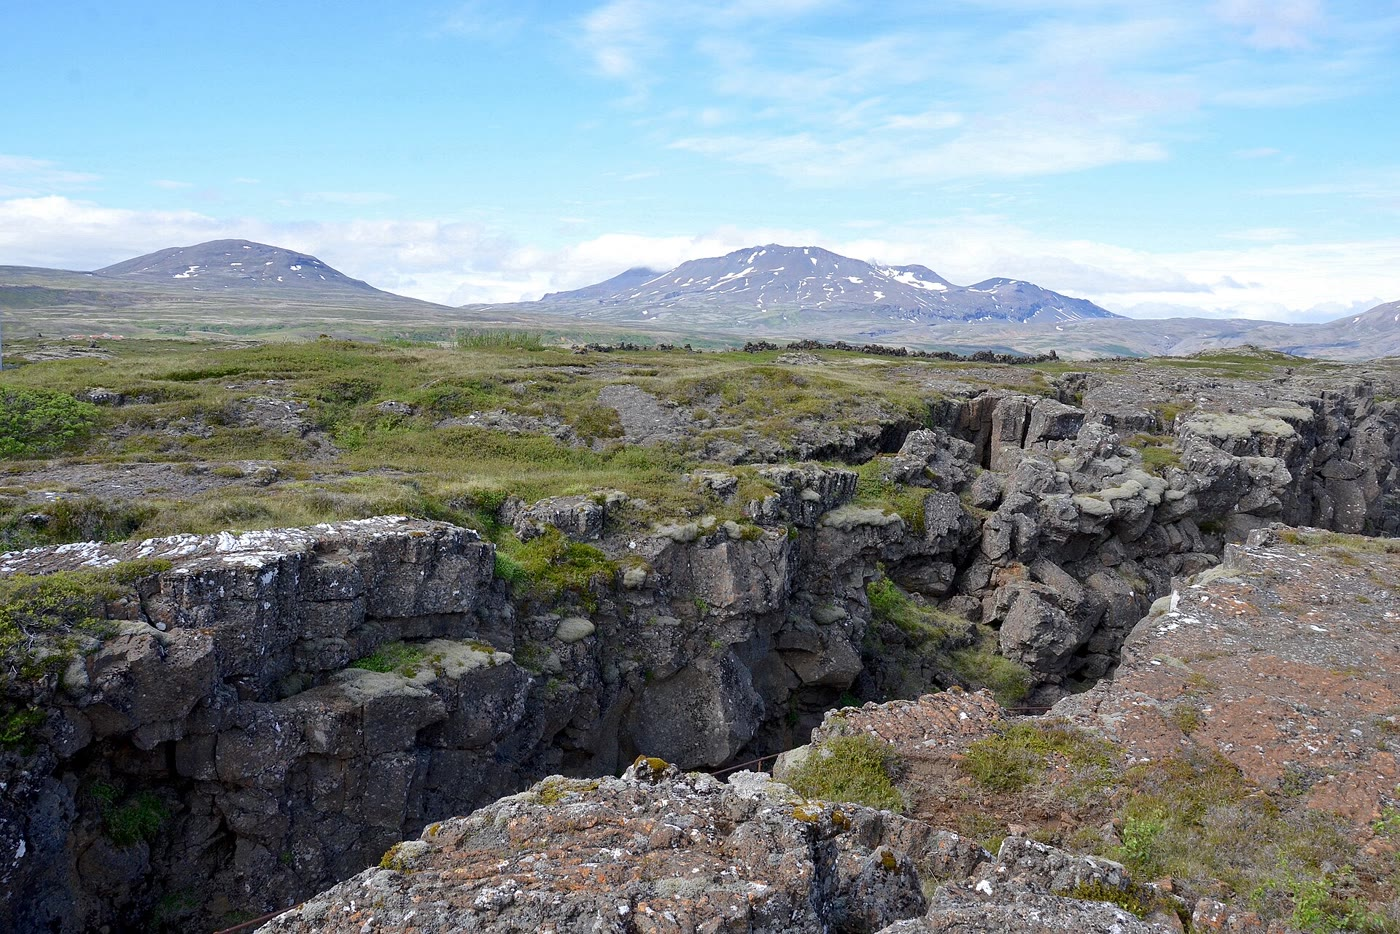
\includegraphics[width=0.8\linewidth]{images/book3/b1-thingvellir-fissure.jpg}

\par\smallskip{\small 辛格维利尔裂谷谷底熔岩地面上的一条张开裂缝，
位于冰岛西南部，中大西洋洋脊在此登陆。
谷底的玄武岩流被与裂谷平行的张开裂缝切割。
照片：Olga Ernst,
CC~BY-SA~4.0（维基共享资源）。}
\label{fig:b1:rifts-ridges-margins:thingvellir}
\end{omfigure}
% ledger: commons:thingvellir

\subsection*{火山型裂谷与贫岩浆裂谷}

裂谷所接收的岩浆多寡不一。在\emph{贫岩浆}裂谷中，
伸展由断层承担，\omterm{def:b1:layered-earth:layers}{地壳}随断块
相互滑开而变薄。在火山型裂谷中，岩浆起主导作用：岩墙沿轴线侵入\omterm{def:b1:layered-earth:layers}{地壳}，
每一条岩墙都以其自身的厚度张开裂谷，熔岩则漫流于地表。
东非裂谷两种类型并存：其东支强烈火山化，
而其西支火山活动较弱，却拥有深厚的沉积盆地，
盆地中充填着坦噶尼喀湖等湖泊，
并以断层为界。
% ledger: roberts:ear

两支大约在 2500 万年前开始形成，裂谷将非洲板块
分割为西侧的努比亚板块与东侧的索马里板块。
从阿法尔\omterm{def:b1:plate-kinematics:triple-junction}{三联点}向南延伸，分为两支，绕过古老、厚重而寒冷的
坦桑尼亚克拉通。其运动十分缓慢：根据索马里板块与努比亚板块各自
相对于南极板块的板块矢量计算，索马里以 \qty{6.0}{mm.\text{年}^{-1}} 的速率
远离努比亚，方向为 \ang{105}，位于埃塞俄比亚中部
（北纬 \ang{8.5}，东经 \ang{39.5}），在赤道上则以
\qty{5.1}{mm.\text{年}^{-1}} 的速率远离。裂谷中的许多地震
显示为正断层型破裂。
% ledger: roberts:ear, morvel:sm-an, morvel:nb-an (SM-NB from SM-AN minus NB-AN, computed with figdata/bachelor-1/euler_velocities.py)

在北端的阿法尔，裂谷与红海和亚丁湾相交。
埃塞俄比亚的大部分洪水玄武岩正是在那里于约 3000 万年前喷发，
历时不超过一百万年；此后岩浆仍不断涌入：熔岩
流溢于地表，侵入体遍布\omterm{def:b1:layered-earth:layers}{地壳}，并在其下方不断增添新物质，
以至于被侵入的\omterm{def:b1:layered-earth:layers}{地壳}在裂谷早期阶段仍保持原有厚度。
2005 年的危机揭示了这类裂谷的张开方式：并非平稳进行，而是
分阶段发生，每一阶段都是宽数米的岩墙在数日或数周之内侵入。既然那里的
板块以约 \qty{18}{mm.\text{年}^{-1}} 的速率分离，则 2005 年那条 \qty{8}{m} 的岩墙
承担了约 440 年的伸展量。
% ledger: hofmann:traps, bastow:afar, wright:afar, morvel:ar-nb (rate computed with euler_velocities.py)

\section{断裂与被动大陆边缘}

若拉伸持续进行，大陆\omterm{def:b1:layered-earth:layers}{地壳}被减薄至零，\omterm{def:b1:layered-earth:layers}{地幔}
在裂谷之下上涌并在上涌过程中发生熔融，于是大陆两半之间形成最初的\omterm{def:b1:rifts-ridges-margins:oceanic-crust}{洋壳}。
这一时刻即为
\emph{断裂}。此后，板块在新海洋中央的洋脊处相互分离，
大陆的两个边缘被带离洋脊，
不再是板块边界。

\begin{definition}[被动大陆边缘、洋陆过渡带、断裂不整合]\label{def:b1:rifts-ridges-margins:passive-margin}
\emph{被动大陆边缘}\index{被动大陆边缘}是由裂谷作用形成、
已不再是板块边界的大陆边缘：大陆与相邻洋底
属于同一板块。
\emph{洋陆过渡带}\index{洋陆过渡带}是
边缘的一个带，宽度为数千米至数十千米，位于减薄的
大陆\omterm{def:b1:layered-earth:layers}{地壳}与正常\omterm{def:b1:rifts-ridges-margins:oceanic-crust}{洋壳}之间。\emph{断裂
不整合}\index{断裂不整合}是将裂谷盆地中沉积并随断块倾斜的沉积物，与
断裂后覆盖于边缘、未受扰动的沉积物
分隔开的\omterm{def:b1:cross-sections:unconformity}{不整合}。
\end{definition}

\omterm{def:b1:rifts-ridges-margins:passive-margin}{被动大陆边缘}分布于大西洋、北冰洋和西印度洋的大部分岸线，
以及非洲、澳大利亚、格陵兰和印度几乎全部的海岸。
北美洲东缘与非洲西北缘曾是同一条裂谷的两侧：
它们互为\emph{共轭}边缘。其剖面
呈现近岸洋底的常见序列：大陆架、陆坡、
陆隆和深海平原。大陆架和陆坡之下是减薄的大陆\omterm{def:b1:layered-earth:layers}{地壳}，
被\omterm{def:b1:geological-maps:attitude}{倾向}洋方向的正断层切割，其旋转的断块
埋藏于沉积物之下。

\begin{omfigure}
\begin{tikzpicture}[x=0.95cm, y=0.9cm, font=\scriptsize]
% (a) continental rift: half-grabens on east-dipping faults; coordinates from calc/fig13_margin.py
\begin{scope}
\fill[green!25!gray!45] (0,-2) -- (3,-2) -- (6,-1.75) -- (9,-2) -- (12,-2) -- (12,-2.5) -- (0,-2.5) -- cycle;
\fill[orange!22] (0,0) -- (3.5,0) -- (3.931,-0.8) -- (4.75,-0.25) -- (5.05,-0.7) -- (6,-0.2) -- (6.223,-0.55) -- (7.25,-0.15) -- (7.402,-0.4) -- (8.6,0) -- (12,0) -- (12,-2) -- (9,-2) -- (6,-1.75) -- (3,-2) -- (0,-2) -- cycle;
\fill[yellow!45] (3.565,-0.12) -- (3.931,-0.8) -- (4.75,-0.25) -- (4.75,-0.12) -- cycle;
\fill[yellow!45] (4.75,-0.12) -- (4.75,-0.25) -- (5.05,-0.7) -- (6,-0.2) -- (6,-0.12) -- cycle;
\fill[yellow!45] (6,-0.12) -- (6,-0.2) -- (6.223,-0.55) -- (7.25,-0.15) -- (7.25,-0.12) -- cycle;
\fill[yellow!45] (7.25,-0.12) -- (7.25,-0.15) -- (7.402,-0.4) -- (8.241,-0.12) -- cycle;
\draw (0,0) -- (3.5,0) -- (3.931,-0.8) -- (4.75,-0.25) -- (5.05,-0.7) -- (6,-0.2) -- (6.223,-0.55) -- (7.25,-0.15) -- (7.402,-0.4) -- (8.6,0) -- (12,0);
\draw[contact] (0,-2) -- (3,-2) -- (6,-1.75) -- (9,-2) -- (12,-2);
\draw[fault] (3.5,0) -- (4.2,-1.3);
\draw[fault] (4.75,-0.25) -- (5.45,-1.3);
\draw[fault] (6,-0.2) -- (6.7,-1.3);
\draw[fault] (7.25,-0.15) -- (7.95,-1.3);
\node[anchor=west, font=\small\bfseries] at (0,0.75) {(a) 大陆裂谷};
\node[anchor=south] at (2.2,0) {裂谷肩};
\node[anchor=south, align=center] at (6.3,0) {充填沉积物的半地堑};
\draw[-{Stealth[length=3pt]}] (2.6,-0.75) node[anchor=east] {边界断层} -- (3.75,-0.5);
\node at (9.8,-1.0) {大陆地壳};
\node at (10.3,-2.25) {地幔};
\node at (6,-2.18) {裂谷下方莫霍面抬升};
\end{scope}
% (b) break-up: conjugate halves, the first oceanic crust between them
\begin{scope}[yshift=-3.6cm]
\fill[omSea!35] (2.8,0) -- (9.2,0) -- (9.2,-1.3) -- (2.8,-1.3) -- cycle;
\fill[green!25!gray!45] (0,-2) -- (2.5,-2) -- (5.5,-1.3) -- (6.5,-1.3) -- (9.5,-2) -- (12,-2) -- (12,-2.5) -- (0,-2.5) -- cycle;
\fill[orange!22] (0,0) -- (2.8,0) -- (3.146,-0.75) -- (3.8,-0.3) -- (4.13,-0.85) -- (4.7,-0.45) -- (5.053,-0.95) -- (5.5,-1) -- (5.5,-1.3) -- (2.5,-2) -- (0,-2) -- cycle;
\fill[orange!22] (12,0) -- (9.2,0) -- (8.854,-0.75) -- (8.2,-0.3) -- (7.87,-0.85) -- (7.3,-0.45) -- (6.947,-0.95) -- (6.5,-1) -- (6.5,-1.3) -- (9.5,-2) -- (12,-2) -- cycle;
\fill[lith basalt] (5.5,-1) -- (6.5,-1) -- (6.5,-1.3) -- (5.5,-1.3) -- cycle;
\draw (0,0) -- (2.8,0) -- (3.146,-0.75) -- (3.8,-0.3) -- (4.13,-0.85) -- (4.7,-0.45) -- (5.053,-0.95) -- (5.5,-1) -- (6.5,-1) -- (6.947,-0.95) -- (7.3,-0.45) -- (7.87,-0.85) -- (8.2,-0.3) -- (8.854,-0.75) -- (9.2,0) -- (12,0);
\draw[contact] (0,-2) -- (2.5,-2) -- (5.5,-1.3) -- (6.5,-1.3) -- (9.5,-2) -- (12,-2);
\draw[omSea!70!black] (2.8,0) -- (9.2,0);
\draw[fault] (2.8,0) -- (3.4,-1.3);
\draw[fault] (3.8,-0.3) -- (4.4,-1.3);
\draw[fault] (4.7,-0.45) -- (5.3,-1.3);
\draw[fault] (9.2,0) -- (8.6,-1.3);
\draw[fault] (8.2,-0.3) -- (7.6,-1.3);
\draw[fault] (7.3,-0.45) -- (6.7,-1.3);
\draw[omRidge, very thick, -{Stealth[length=3pt]}] (6,-2.3) -- (6,-1.45);
\node[anchor=west, font=\small\bfseries] at (0,0.75) {(b) 断裂};
\node[anchor=south] at (6,0) {海水淹没裂谷};
\node[anchor=west] at (6.15,-2.1) {地幔上涌并熔融};
\node[anchor=south, fill=white, fill opacity=0.8, text opacity=1, inner sep=1pt, align=center] at (6,-0.85) {最初的 \\洋壳};
\node at (1.4,-1.0) {倾斜断块};
\node at (10.6,-1.0) {倾斜断块};
\node at (1.4,-2.25) {地幔};
\end{scope}
% (c) one passive margin after drift
\begin{scope}[yshift=-7.4cm]
\fill[omSea!35] (1.2,0.3) -- (12,0.3) -- (12,-1.2) -- (8.2,-1.15) -- (6.4,-0.9) -- (4.6,0.1) -- cycle;
\fill[green!25!gray!45] (0,-2.3) -- (2,-2.3) -- (5.9,-1.8) -- (6.7,-2.1) -- (12,-2.1) -- (12,-2.7) -- (0,-2.7) -- cycle;
\fill[orange!22] (0,0.3) -- (1.2,0.3) -- (2.2,0) -- (3,-0.25) -- (3.259,-0.95) -- (4,-0.55) -- (4.286,-1.15) -- (4.9,-0.85) -- (5.233,-1.35) -- (5.9,-1.55) -- (5.9,-1.8) -- (2,-2.3) -- (0,-2.3) -- cycle;
\fill[pattern=crosshatch dots, pattern color=green!40!black] (5.9,-1.55) -- (6.4,-1.75) -- (6.7,-2.1) -- (5.9,-1.8) -- cycle;
\fill[lith basalt] (6.4,-1.75) -- (12,-1.75) -- (12,-2.1) -- (6.7,-2.1) -- cycle;
\fill[yellow!45] (3,-0.25) -- (3.259,-0.95) -- (4,-0.55) -- cycle;
\fill[yellow!45] (4,-0.55) -- (4.286,-1.15) -- (4.9,-0.85) -- cycle;
\fill[yellow!45] (4.9,-0.85) -- (5.233,-1.35) -- (5.9,-1.55) -- (5.9,-1.45) -- cycle;
\fill[yellow!15] (1.2,0.3) -- (4.6,0.1) -- (6.4,-0.9) -- (8.2,-1.15) -- (12,-1.2) -- (12,-1.75) -- (6.4,-1.75) -- (5.9,-1.55) -- (5.9,-1.45) -- (4.9,-0.85) -- (4,-0.55) -- (3,-0.25) -- (2.2,0) -- cycle;
\draw[black!45] (2.4,0.12) -- (4.8,-0.1) -- (6.6,-1.05) -- (8.4,-1.27) -- (12,-1.31);
\draw (1.2,0.3) -- (4.6,0.1) -- (6.4,-0.9) -- (8.2,-1.15) -- (12,-1.2);
\draw[omSea!70!black] (1.2,0.3) -- (12,0.3);
\draw[unconformity] (2.2,0) -- (3,-0.25) -- (4,-0.55) -- (4.9,-0.85) -- (5.9,-1.45);
\draw (3.259,-0.95) -- (4,-0.55) (4.286,-1.15) -- (4.9,-0.85) (5.233,-1.35) -- (5.9,-1.55) -- (6.4,-1.75) -- (12,-1.75);
\draw[contact] (0,-2.3) -- (2,-2.3) -- (5.9,-1.8) -- (6.7,-2.1) -- (12,-2.1);
\draw[fault] (3,-0.25) -- (3.5,-1.6);
\draw[fault] (4,-0.55) -- (4.5,-1.6);
\draw[fault] (4.9,-0.85) -- (5.4,-1.6);
\node[anchor=west, font=\small\bfseries] at (0,0.95) {(c) 被动大陆边缘};
\node[anchor=south] at (3.4,0.25) {陆架};
\node[anchor=south west] at (5.6,-0.45) {陆坡};
\node[anchor=south] at (8.4,-1.12) {陆隆};
\node[anchor=south] at (10.6,-1.17) {深海平原};
\node[anchor=south] at (10.6,-0.1) {海洋};
\node at (9.8,-1.53) {裂后沉积物};
\node[fill=white, fill opacity=0.8, text opacity=1, inner sep=1pt, align=center] (bu) at (1.0,-0.6) {断裂 \\不整合};
\draw[-{Stealth[length=3pt]}] (bu.east) -- (2.55,-0.16);
\node[fill=white, fill opacity=0.8, text opacity=1, inner sep=1pt, align=center] (sr) at (1.6,-1.35) {同裂谷 \\沉积物};
\draw[-{Stealth[length=3pt]}] (sr.east) -- (3.45,-0.75);
\node at (1.3,-1.98) {大陆地壳};
\draw[decorate, decoration={brace, amplitude=3pt, mirror}] (5.9,-2.17) -- (6.7,-2.17) node[midway, below=3pt, align=center] {洋陆 \\过渡带};
\node[anchor=west, fill=white, fill opacity=0.85, text opacity=1, inner sep=1pt] at (8.6,-1.93) {洋壳};
\node at (3.6,-2.5) {地幔};
\end{scope}
\end{tikzpicture}

\par\smallskip{\small 从裂谷到\omterm{def:b1:rifts-ridges-margins:passive-margin}{被动大陆边缘}（示意图，不按比例；
高度经过夸大）。(a) 脆性上\omterm{def:b1:layered-earth:layers}{地壳}沿
正断层断裂；块体倾斜成\omterm{def:b1:rifts-ridges-margins:rift}{半地堑}并充填沉积物，\omterm{def:b1:layered-earth:discontinuity}{莫霍面}
在减薄的\omterm{def:b1:layered-earth:layers}{地壳}之下抬升。(b) 裂解时陆壳被切穿，
海水淹没裂谷，形成最初的\omterm{def:b1:rifts-ridges-margins:oceanic-crust}{洋壳}。(c) 两个
大陆边缘之一随离开洋脊而被带走：其倾斜块体及其
沉积物位于裂解\omterm{def:b1:cross-sections:unconformity}{不整合}之下，被陆架、陆坡与陆隆的
裂后沉积物掩埋。}
\label{fig:b1:rifts-ridges-margins:margin}
\end{omfigure}

\subsection*{两类大陆边缘}

大陆边缘继承了其裂谷的性质。在\emph{贫岩浆型}
大陆边缘（如伊比利亚和纽芬兰的边缘）上，地震剖面显示旋转的
块体，其岩层向陆倾斜；局部地区，\omterm{def:b1:rifts-ridges-margins:passive-margin}{洋陆过渡带}
底部为\omterm{def:b1:layered-earth:layers}{地幔}橄榄岩，被抬升至海底并
被海水蚀变为蛇纹岩。在\emph{火山型}大陆边缘（如
挪威中部、东格陵兰、纳米比亚与巴西的边缘）上，过渡带
由玄武岩构成：向洋倾斜的熔岩流层序、
地震剖面中向海倾斜的反射体，其下为下\omterm{def:b1:layered-earth:layers}{地壳}，
其中 P 波传播异常快，岩浆在
裂解时加入\omterm{def:b1:layered-earth:layers}{地壳}之下。火山型大陆边缘在裂解期间下沉甚微。

\begin{inthefield}[寻找大陆的边缘]
\omterm{def:b1:rifts-ridges-margins:passive-margin}{洋陆过渡带}位于数千米的水体和沉积物之下，
只能借助地球物理方法定位，通常需要多种方法联合使用。
地震反射可成像倾斜块体、裂解\omterm{def:b1:cross-sections:unconformity}{不整合}，以及
信号足够深时的\omterm{def:b1:layered-earth:discontinuity}{莫霍面}。广角地震折射
测量 P 波穿过\omterm{def:b1:layered-earth:layers}{地壳}的速度，二者在
陆壳与\omterm{def:b1:rifts-ridges-margins:oceanic-crust}{洋壳}之间有所不同。重力数据经反演求取\omterm{def:b1:layered-earth:discontinuity}{莫霍面}深度，
从而给出\omterm{def:b1:layered-earth:layers}{地壳}厚度。洋底的磁条带
在磁性平静的陆壳出现处中止。
\end{inthefield}

裂解之后，大陆边缘下沉。裂谷作用期间，\omterm{def:b1:layered-earth:lithosphere}{岩石圈}变薄并
被加热；离开洋脊后冷却收缩，如同其旁的洋底，
上方张开的空间被裂后沉积物楔
充填，其重量使之进一步下沉。这一过程的冷却部分
见\cref{sec:b1:rifts-ridges-margins:depth-age}；沉积物的
重量则在\cref{ch:b1:diagenesis-basins}中讨论。

\section{快速与慢速洋脊}

洋盆形成之后，便在其洋脊处持续生长。洋脊的扩张
速率差异很大：过去数百万年测得的速率从
北红海的\qty{9.7}{mm.\text{年}^{-1}}，到东太平洋海隆的
\qty{154.4}{mm.\text{年}^{-1}}。洋脊的形态取决于该速率。
% ledger: morvel:range

\begin{definition}[快速、慢速与超慢速扩张洋脊]\label{def:b1:rifts-ridges-margins:ridge-classes}
洋脊按其\omterm{def:b1:plate-kinematics:spreading-rate}{全扩张速率}分类。
\emph{超慢速扩张洋脊}\index{超慢速扩张洋脊}的\omterm{def:b1:plate-kinematics:spreading-rate}{全扩张
速率}低于约\qty{20}{mm.\text{年}^{-1}}；\emph{慢速扩张
洋脊}\index{慢速扩张洋脊}的速率为 20 至\qty{55}{mm.\text{年}^{-1}}；
中间型洋脊为 55 至\qty{75}{mm.\text{年}^{-1}}；\emph{快速扩张
洋脊}\index{快速扩张洋脊}的速率超过约
\qty{75}{mm.\text{年}^{-1}}。
\end{definition}
% ledger: seton:rate-classes, dick:ultraslow

这些界限只是约定，不同作者取值不一。不变的是
形态的变化。慢速洋脊，如大西洋中脊，
在相向的正断层之间有一轴谷：两板块之间的
空隙不能像其张开那样迅速被岩浆充填，冷的\omterm{def:b1:layered-earth:lithosphere}{岩石圈}
破裂。快速洋脊，如东太平洋海隆，没有裂谷，而是
轴部呈平滑隆起，其下有透镜状熔体，补给足够频繁以跟上扩张。
无论哪种情况，洋脊轴的深度约为\qty{2500}{m}，而
盆地中最老的洋底比其深近\qty{4}{km}（见\cref{sec:b1:rifts-ridges-margins:depth-age}）。
% ledger: parsons:plate-model (6400 - 2500 m)

超慢速洋脊显示了岩浆最匮乏时的情形：其火山活动
间歇性的，缺少\omterm{def:b1:rifts-ridges-margins:transform}{转换断层}，并在大范围内\omterm{def:b1:layered-earth:layers}{地幔}
本身被抬升至海底。位于北冰洋下的加克尔洋脊，
是所有洋脊中扩张最慢者，完全未被错断；沿其轴部的中段
约\qty{300}{km}长的一段，\omterm{def:b1:layered-earth:layers}{地幔}橄榄岩直接位于轴上，
西侧是密集的火山活动，东侧是
大型、间距较大的火山。在慢速与超慢速洋脊上尤甚，部分扩张
由长而缓倾的拆离断层承担，其下盘
从轴下被拉出：辉长岩与橄榄岩以
波状穹隆之形出露于海底，形成\emph{洋底核杂岩}。亚特兰蒂斯地块位于
在北纬 \ang{30} 附近的大西洋中脊旁，是其中之一：其顶部位于
距轴约\qty{15}{km}、年龄约\qty{1.5}{Ma}的\omterm{def:b1:rifts-ridges-margins:oceanic-crust}{洋壳}上，海水与
\omterm{def:b1:layered-earth:layers}{地幔}岩反应，形成失落之城
热液区的温热碱性泉。
% ledger: dick:ultraslow, michael:gakkel, kelley:lost-city

\subsection*{洋壳}

\begin{definition}[洋壳、枕状熔岩与席状岩墙群]\label{def:b1:rifts-ridges-margins:oceanic-crust}
\emph{洋壳}\index{洋壳}是在洋脊处形成的\omterm{def:b1:layered-earth:layers}{地壳}，
自海底向下至\omterm{def:b1:layered-earth:discontinuity}{莫霍面}，厚 6 至\qty{7}{km}，由玄武岩和辉长岩组成，
其上覆有沉积物。\emph{枕状熔岩}\index{枕状熔岩}是
在水下喷出的熔岩，由圆形且相互连通的管状体与瓣状体组成，每个
均具有被海水冷却的玻璃质外壳。\emph{席状岩墙
群}\index{席状岩墙群}是几乎完全由
平行直立岩墙组成的层，每条岩墙侵入先前的岩墙之中。
\end{definition}

\omterm{def:b1:rifts-ridges-margins:oceanic-crust}{洋壳}各层最初由地震学界定，随后经钻探取样，
并在逆冲至大陆之上的洋底岩片中得到识别，
即蛇绿岩。自上而下依次为：
\begin{itemize}
  \item 第~1~层，沉积物，靠近洋脊处薄或缺失，并随
        洋底年龄增大而增厚；
  \item 第~2~层，平均厚\qty{1.84}{km}的玄武岩：顶部为\omterm{def:b1:rifts-ridges-margins:oceanic-crust}{枕状熔岩}
        （第~2A~层），其下为辉绿岩席状岩墙（第~2B~层）；
  \item 第~3~层，其余 4 至 5 千米，主要为辉长岩，其
        底部为从岩浆中沉降堆积的堆晶岩：约占
        \omterm{def:b1:layered-earth:layers}{地壳}厚度的\qty{70}{\percent}。
\end{itemize}
\omterm{def:b1:layered-earth:discontinuity}{莫霍面}之下为\omterm{def:b1:layered-earth:layers}{地幔}橄榄岩，是熔融后的残余物。
% ledger: christeson:crust, white:crust (layer 3: 6.15 - 1.84 = 4.3 km, 70 %; 7.1 - 1.84 = 5.3 km)

地震折射给出火成\omterm{def:b1:layered-earth:layers}{地壳}的平均厚度，
在远离断裂带和热点处为\qty[uncertainty-mode=separate]{7.1 \pm 0.8}{km}；
后来对地震剖面的综合分析给出\qty{6.15}{km}，各扩张速率下大致相同：
熔体的量取决于上涌\omterm{def:b1:layered-earth:layers}{地幔}的温度，而不取决于其上升速度。
只有极慢速的洋脊才形成异常薄的\omterm{def:b1:layered-earth:layers}{地壳}：
那里的\omterm{def:b1:layered-earth:layers}{地幔}在上升过程中有足够时间冷却，熔融程度也较低。
在热柱上方\omterm{def:b1:layered-earth:layers}{地壳}较厚，在上升热柱的核心正上方约为\qty{20}{km}，
冰岛之下即是如此（见\cref{ch:b1:hotspots}）。
所有洋脊合计，每年
约生成\qty{3.0}{km^2}的新洋底，
以及约\qty{20}{km^3}的新\omterm{def:b1:layered-earth:layers}{地壳}。
% ledger: white:crust, christeson:crust, data:pb2002 (production summed over the spreading steps in figdata/bachelor-1/ridge_budget.py)

\begin{omfigure}
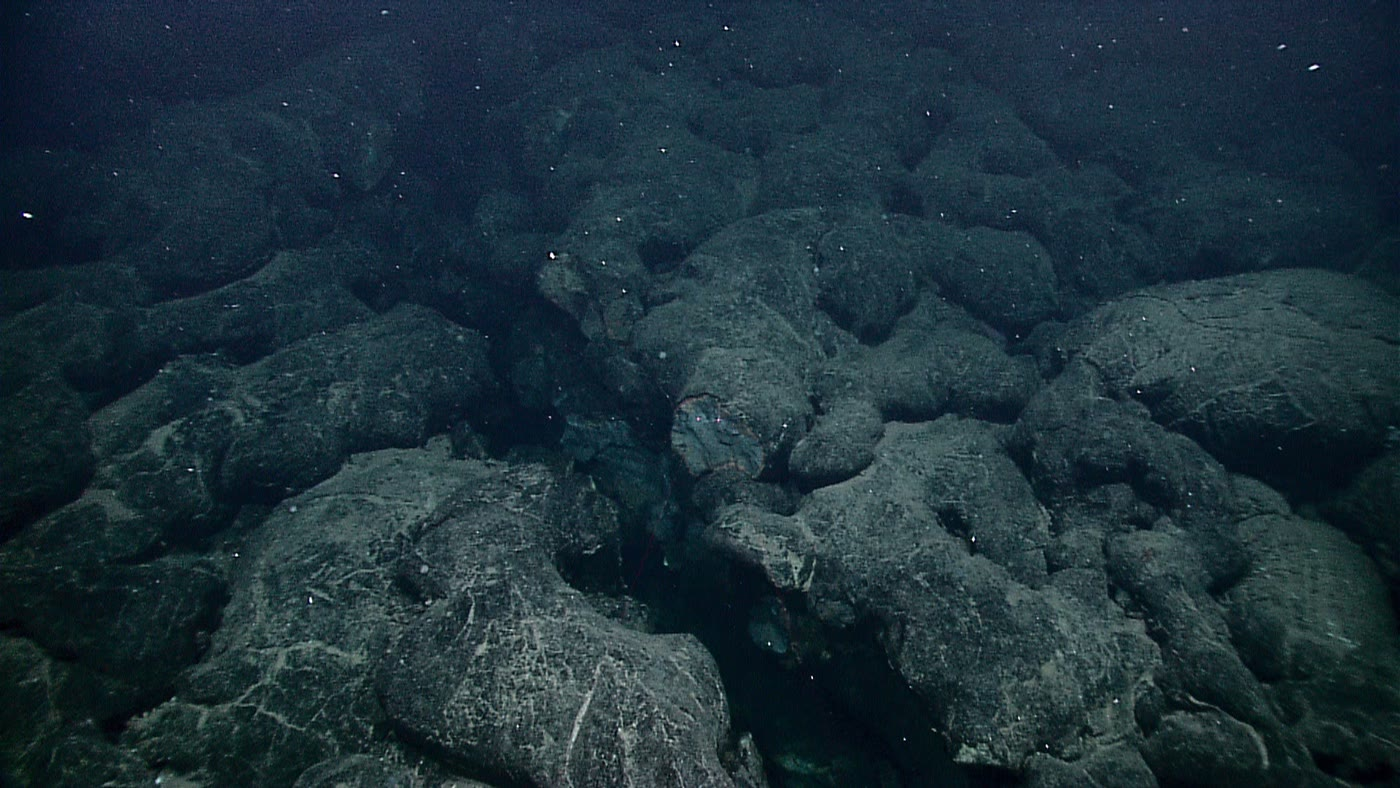
\includegraphics[width=0.6\linewidth]{images/book3/b1-pillow-lava.jpg}

\par\smallskip{\small 加拉帕戈斯裂谷的\omterm{def:b1:rifts-ridges-margins:oceanic-crust}{枕状熔岩}，被一条在其凝固后才张开的裂隙切穿，
即正在形成中的\omterm{def:b1:rifts-ridges-margins:oceanic-crust}{洋壳}第~2~层的顶部：
每个枕状体都是一股熔岩舌，其外部被
海水冷凝而成。照片：NOAA Okeanos Explorer Program, Galápagos Rift Expedition
2011，CC~BY~2.0（维基共享资源）。}
\label{fig:b1:rifts-ridges-margins:pillows}
\end{omfigure}
% ledger: commons:pillow-expl6453

\begin{proposition}[每条岩墙都切分其前一条]\label{prop:b1:rifts-ridges-margins:dykes}
假设\omterm{def:b1:rifts-ridges-margins:oceanic-crust}{席状岩墙群}中的每条岩墙都沿扩张轴侵入，
扩张轴处\omterm{def:b1:layered-earth:layers}{地壳}最热、最弱，且\omterm{def:b1:layered-earth:layers}{地壳}对称地远离轴线运动。
则大多数岩墙被发现已一分为二，
每一半仅在与其较老邻居相接的一侧具有冷凝边缘。
\end{proposition}

\begin{proof}
岩墙在两侧较冷的岩石处冷却：形成时它具有
两个冷凝边缘。下一条岩墙沿轴线、在\omterm{def:b1:layered-earth:layers}{地壳}最弱处上升，
即穿过前一条岩墙的中部，那里仍是最热的岩石。
它将前一条岩墙切为两半，扩张将两半分别带向两侧；
每一半外侧保留冷凝边缘，
内侧则与新岩墙有一未冷却的接触面。
除最后一条外，每条岩墙都以此方式被切分。
\end{proof}

只在一侧带有冷凝边缘的岩墙，确实是\omterm{def:b1:rifts-ridges-margins:oceanic-crust}{席状岩墙群}的常见情形：
这正是\omterm{def:b1:layered-earth:layers}{地壳}逐条岩墙堆叠而成的标志，
其堆叠动力即为扩张。


\section{深度–年龄关系}\label{sec:b1:rifts-ridges-margins:depth-age}

洋底在洋脊处较浅，远离洋脊处较深。由于洋底在洋脊处生成并被带走，
离洋脊的距离即是年龄，洋底的深度
取决于其年龄。板块随年龄增长从上方冷却
（见\cref{ch:b1:heat-budget}）；冷岩石密度更大，密度更大的柱体漂浮
得更低。

\begin{lemma}[误差函数的一个积分]\label{lem:b1:rifts-ridges-margins:erfc}
记 $\operatorname{erfc} u = 1 - \operatorname{erf} u =
\frac{2}{\sqrt\pi}\int_u^\infty e^{-s^2}\,\mathrm ds$,
\[
  \int_0^\infty \operatorname{erfc} u \,\mathrm du = \frac{1}{\sqrt\pi}.
\]
\end{lemma}

\begin{proof}
$\operatorname{erfc}$ 的导数为 $-\frac{2}{\sqrt\pi}e^{-u^2}$。
在 $[0, X]$ 上分部积分，
\[
  \int_0^X \operatorname{erfc} u\,\mathrm du
  = \bigl[u \operatorname{erfc} u\bigr]_0^X + \frac{2}{\sqrt\pi}\int_0^X u\,e^{-u^2}\,\mathrm du
  = X\operatorname{erfc} X + \frac{1}{\sqrt\pi}\bigl(1 - e^{-X^2}\bigr).
\]
当 $X > 0$ 且 $s \ge X$ 时，$e^{-s^2} \le (s/X)e^{-s^2}$，于是
$X\operatorname{erfc} X \le \frac{2}{\sqrt\pi}\int_X^\infty s\,e^{-s^2}\,\mathrm ds
= e^{-X^2}/\sqrt\pi$ 趋于 0，令 $X \to \infty$，
即得所证。
\end{proof}

\begin{theorem}[深度–年龄关系]\label{thm:b1:rifts-ridges-margins:depth-age}
假设
\begin{enumerate}
  \item \omterm{def:b1:layered-earth:layers}{地幔}以均匀温度 $T_m$ 离开洋脊，并且
        年龄为 $t$ 的洋板块是一个自那时起从其表面开始冷却的半空间，
        表面保持在 $T_0$，热扩散率为 $\kappa$；
  \item 冷却岩石的密度为 $\rho_m\bigl(1 + \alpha(T_m -
        T)\bigr)$，其中 $\rho_m$ 为 $T_m$ 时\omterm{def:b1:layered-earth:layers}{地幔}的密度，
        $\alpha$ 为其热膨胀系数；
  \item 每个柱体都处于\omterm{def:b1:isostasy-gravity:isostasy}{地壳均衡}状态，其\omterm{def:b1:isostasy-gravity:isostasy}{补偿深度}
        位于冷却层之下，海水的密度为 $\rho_w$。
\end{enumerate}
于是年龄为 $t$ 的洋底深度为
\[
  d(t) = d_r + C\sqrt t, \qquad
  C = \frac{2}{\sqrt\pi}\,\frac{\rho_m\,\alpha\,(T_m - T_0)\sqrt\kappa}{\rho_m - \rho_w},
\]
其中 $d_r$ 为洋脊轴的深度。此即洋底的
\emph{深度–年龄关系}\index{深度–年龄关系}。
\end{theorem}

\begin{proof}
冷却半空间中的温度为
\[
  T(z, t) = T_0 + (T_m - T_0)\operatorname{erf}\frac{z}{2\sqrt{\kappa t}},
\]
其中 $z$ 为洋底以下的深度；此热传导方程的解与
在\cref{ch:b1:heat-budget}中一样，在本阶段不加证明地承认，其推导见本科三年级分册。
比较洋脊处的柱体：其上为深至 $d_r$ 的海水，
其下为温度 $T_m$ 的\omterm{def:b1:layered-earth:layers}{地幔}；与年龄为 $t$ 的柱体相比，其上为深至 $d$ 的海水，
其下为冷却的板块，两者均延伸至\omterm{def:b1:isostasy-gravity:isostasy}{补偿深度} $D$。二者单位面积上的质量
相等：
\[
  \rho_w d_r + \rho_m (D - d_r) = \rho_w d + \int_0^{D-d}\rho_m\bigl(1 + \alpha(T_m - T)\bigr)\mathrm dz
  = \rho_w d + \rho_m (D - d) + \rho_m\alpha\int_0^{D-d}(T_m - T)\,\mathrm dz.
\]
由此
\[
  (\rho_m - \rho_w)(d - d_r) = \rho_m\alpha\int_0^{D-d}(T_m - T)\,\mathrm dz.
\]
由于 $T_m - T = (T_m - T_0)\operatorname{erfc}\bigl(z/2\sqrt{\kappa t}\bigr)$ 在
冷却层之下可以忽略，故积分可取至无穷；令
$u = z/2\sqrt{\kappa t}$，并利用\cref{lem:b1:rifts-ridges-margins:erfc}，
\[
  \int_0^\infty (T_m - T)\,\mathrm dz = (T_m - T_0)\,2\sqrt{\kappa t}\int_0^\infty\operatorname{erfc}u\,\mathrm du
  = \frac{2}{\sqrt\pi}(T_m - T_0)\sqrt{\kappa t}.
\]
除以 $\rho_m - \rho_w$ 即得 $d - d_r = C\sqrt t$。
\end{proof}

水的影响不可忽略：板块下沉时，水充满其上方的空间，
水的重量把板块进一步压低。有效膨胀系数
$\alpha\rho_m/(\rho_m - \rho_w)$ 较 $\alpha$ 大，倍数为
$3300/2300 \approx 1.43$。

取 $\alpha = \qty{3.2e-5}{K^{-1}}$，$T_m - T_0 = \qty{1350}{K}$，
$\kappa = \qty{e-6}{m^2.s^{-1}}$，$\rho_m = \qty{3300}{kg.m^{-3}}$ 及
$\rho_w = \qty{1000}{kg.m^{-3}}$，时间以百万年计
（$\sqrt{\kappa\times\qty{1}{Ma}} = \qty{5618}{m}$），由定理得
$C = \qty{393}{m.Ma^{-1/2}}$。帕森斯和斯克拉特对北太平洋与北大西洋的
洋底深度作拟合，去除沉积物之后，两者相当接近：
$d_r \approx \qty{2500}{m}$ 与
$C \approx \qty{350}{m.Ma^{-1/2}}$，适用于 0 至 \qty{70}{Ma}。
上文中 $\alpha$ 与 $T_m$ 的取值，取自其老洋底板块模型：
\omterm{def:b1:layered-earth:layers}{地幔}温度为 \qty{1350}{\degreeCelsius}，
$\alpha = \qty{3.2e-5}{\per\degreeCelsius}$，二者的不确定度分别为五分之一和三分之一，
因此 393 与 350 的吻合已达到
所能期望的程度。
% ledger: parsons:plate-model, ps77:depth-age

\begin{example}[年龄为 2500 万年和 1 亿年的洋底]\label{ex:b1:rifts-ridges-margins:depths}
由 $d = 2500 + 350\sqrt t$（以米计，$t$ 以百万年计）得，
年龄为 \qty{25}{Ma} 的洋底深度为 $2500 + 350\times5 = \qty{4250}{m}$，
年龄为 \qty{100}{Ma} 的洋底深度为 $2500 + 350\times10 = \qty{6000}{m}$。该洋底
在最初 2500 万年内下沉 \qty{1750}{m}，
而在随后的 7500 万年内仅再下沉 \qty{1750}{m}。
\end{example}
% ledger: parsons:plate-model

\begin{omfigure}
\begin{tikzpicture}
\begin{axis}[omrecord, omdepth, width=0.84\linewidth, height=6.6cm,
  xmin=0, xmax=13.6, ymin=2000, ymax=6800,
  xlabel={洋底年龄的平方根，$\sqrt t$（\unit{Ma^{1/2}}）},
  ylabel={深度（\unit{m}）},
  yticklabel style={/pgf/number format/set thousands separator={}},
  legend style={font=\scriptsize, at={(0.02,0.03)}, anchor=south west, draw=none, fill=white, fill opacity=0.85, text opacity=1},
  legend cell align=left]
% computed in figdata/bachelor-1/depth_age.py; ledger: data:etopo1, data:b2-seafloor-age, parsons:plate-model
\addplot[name path=lo, draw=none, forget plot] table[x expr=sqrt(\thisrow{t}), y=q1] {figdata/out/bachelor-1-depth_age-bins.dat};
\addplot[name path=hi, draw=none, forget plot] table[x expr=sqrt(\thisrow{t}), y=q3] {figdata/out/bachelor-1-depth_age-bins.dat};
\addplot[black!12] fill between[of=lo and hi];
\addlegendentry{网格中间一半}
\addplot[only marks, mark=*, mark size=1.1pt, black!70] table[x expr=sqrt(\thisrow{t}), y=median] {figdata/out/bachelor-1-depth_age-bins.dat};
\addlegendentry{中位深度，2-Ma 年龄区间}
\addplot[very thick, omProp] table[x expr=sqrt(\thisrow{t}), y=halfspace] {figdata/out/bachelor-1-depth_age-models.dat};
\addlegendentry{半空间模型，$2500 + 350\sqrt t$}
\addplot[thick, omDef, densely dashed] table[x expr=sqrt(\thisrow{t}), y=plate] {figdata/out/bachelor-1-depth_age-models.dat};
\addlegendentry{板块模型，$6400 - 3200\,e^{-t/62.8}$}
\draw[black!50, densely dotted] (axis cs:8.944,2000) -- (axis cs:8.944,6800);
\node[font=\scriptsize, anchor=north west, black!70] at (axis cs:8.944,2060) {\qty{80}{Ma}};
\node[font=\scriptsize, anchor=north west, black!70] at (axis cs:4.472,2060) {\qty{20}{Ma}};
\draw[black!50, densely dotted] (axis cs:4.472,2000) -- (axis cs:4.472,6800);
\end{axis}
\end{tikzpicture}

\par\smallskip{\small 洋底深度随其年龄平方根的变化。每个点为世界大洋中
一度网格单元的中位深度，其洋底落在某个两百万年年龄区间内
（共 31\,538 个网格，深度大于
\qty{1000}{m}）；灰色带覆盖其中间一半。半空间定律
在本图中为一条直线。年轻洋底与之十分吻合；较老的洋底
位于其上方，因为这些网格带有沉积物，并包括海山和火山高原，
又因为老洋底停止下沉（虚线为板块模型）。
数据来源：ETOPO1（NOAA）以及塞顿等人
（2020）的洋底年龄数据。}
\label{fig:b1:rifts-ridges-margins:depth-age}
\end{omfigure}

本图在整个大洋上检验了该定理。直至约
\qty{20}{Ma}（$\sqrt t \approx 4.5$）时，中位深度与定律的偏差约在一百
米以内。若对年轻于
\qty{70}{Ma} 的中位深度作直线拟合，其斜率仅为 \qty{250}{m.Ma^{-1/2}}：
所测深度是沉积物表面的深度，而定律给出的是
\omterm{def:b1:layered-earth:layers}{地壳}顶面的深度，且沉积层随年龄增厚。在 60 至
\qty{80}{Ma} 之间，即使去除沉积物，洋底仍偏离平方根定律，
变得比定律所预测的更浅，并停止下沉。
板块模型中，板块厚 \qty{125}{km}，其底部保持在\omterm{def:b1:layered-earth:layers}{地幔}温度，
这一模型描述了这种趋于平缓的现象：其深度趋近于约
\qty{6400}{m}，其\omterm{def:b1:heat-budget:heat-flow}{热流}趋于常数，仿佛热量
由对流\omterm{def:b1:layered-earth:layers}{地幔}输送到老板块底部。该模型在
本科三年级分册中研究；本书中平方根定律仅用于 \qty{80}{Ma} 以内。
% ledger: parsons:plate-model; fit and cell count from depth_age.py (values part)

\begin{method}[由深度确定洋底年龄]\label{met:b1:rifts-ridges-margins:age-from-depth}
在洋底磁异常缺失或未经测绘的地区，
可按下列步骤估算其年龄：
\begin{enumerate}
  \item 测量洋底深度，并由地震剖面测定其沉积层的
        厚度；取\omterm{def:b1:layered-earth:layers}{地壳}顶面的深度 $d$，
        并对沉积物的重量作修正；
  \item 反演定律：$t = \bigl((d - d_r)/C\bigr)^2$，其中 $d_r$ 与 $C$ 取
        所涉大洋的数值；
  \item 检验洋底是否年轻于约 \qty{80}{Ma}，并估算
        不确定度：深度的误差 $\delta d$ 给出
        $\delta t = 2t\,\delta d/(d - d_r)$。
\end{enumerate}
\end{method}

若洋底深度为 \qty{4600}{m}，则 $t = (2100/350)^2 = \qty{36}{Ma}$，而
深度的不确定度为 \qty{100}{m}，由此得年龄的不确定度为 $2\times36\times100/2100 \approx
\qty{3.4}{Ma}$。若洋底在大片区域内比定律预测的更浅，
即所谓的海底隆起，其成因并非年龄，而是来自下方的热量
（见\cref{ch:b1:hotspots}）。

该定律还将大洋与海平面联系起来。扩张较快的洋脊
将年轻而较浅的洋底带离其轴线更远；大洋盆地所容纳的
水减少，海水便漫过大陆而上升。在数千万年的时间尺度上，
扩张速率的变化，是全球海平面变化的两大主因之一，
另一个是陆地冰的体积。

\section{转换断层与破碎带}

洋脊并非连续的线：它们被断层切割成若干段，
这些断层与洋脊成直角、沿扩张方向延伸。越过错开处，
断层仍以长条状痕迹横贯洋底。

\begin{definition}[转换断层，破碎带]\label{def:b1:rifts-ridges-margins:transform}
称\emph{转换断层}\index{转换断层}为一种走滑断层，它是板块边界，
并终止于其他板块边界；洋脊–洋脊转换断层
连接两段错开洋脊段的端点。称\emph{破碎
带}\index{破碎带}为转换断层越过洋脊段端点后的延伸，
即横跨洋底的线状谷地或台阶，
它把同属一个板块、年龄不同的洋底分隔开来。
\end{definition}

\begin{proposition}[洋脊–洋脊转换断层上的滑动]\label{prop:b1:rifts-ridges-margins:transform}
两段洋脊各自以半速率 $u$ 对称扩张，扩张方向与自身垂直，
被一条长度为 $a$ 的\omterm{def:b1:rifts-ridges-margins:transform}{转换断层}错开。则：
\begin{enumerate}
  \item \omterm{def:b1:rifts-ridges-margins:transform}{转换断层}两侧以全速率
        $2u$ 相对错动，其方向与把一条直洋脊切开并由断层错开时
        所暗示的方向相反；
  \item 沿\omterm{def:b1:rifts-ridges-margins:transform}{破碎带}，两侧相对静止，
        两侧洋底的年龄相差 $a/u$；
  \item \omterm{def:b1:rifts-ridges-margins:transform}{转换断层}的长度不随时间变化。
\end{enumerate}
\end{proposition}

\begin{proof}
在洋脊参考系中，取沿\omterm{def:b1:rifts-ridges-margins:transform}{转换断层}、指向东的 $x$ 轴，以及
指向北的 $y$ 轴。设北段位于
$x = 0$，$y > 0$，南段位于 $x = a$，$y < 0$（错开方向是向南时偏向东）；
\omterm{def:b1:rifts-ridges-margins:transform}{转换断层}为线段 $0 < x < a$，位于 $y = 0$ 上。
西侧板块 $W$ 位于两段以西，以 $-u$ 沿 $x$ 方向运动；
东侧板块 $E$ 位于两段以东，以 $+u$ 运动。

(1) 紧邻\omterm{def:b1:rifts-ridges-margins:transform}{转换断层}以北、$0 < x < a$ 处，洋底位于北段以东，
属于板块 $E$，以 $u$ 向东运动。紧邻其以南处，洋底位于
南段以西，属于板块 $W$，以
$u$ 向西运动。北侧相对南侧以 $2u$ 向东运动，
从任一侧看，远侧向右运动，因此这种滑动是右行的。
若一条直洋脊被断层切开，其南段
如今位于北段之东，则记录到的将是左行的
错动。

(2) 当 $x > a$ 时，两侧都位于各自洋脊段之东，且同属 $E$，
二者一起运动。在距北段为 $x$ 处，\omterm{def:b1:rifts-ridges-margins:transform}{破碎带}以北洋底
的年龄为 $x/u$；\omterm{def:b1:rifts-ridges-margins:transform}{破碎带}以南洋底距南段为 $x - a$，年龄为 $(x - a)/u$。
两者之差为 $a/u$。同样的结论对
$x < 0$ 成立，此时两侧都属于 $W$。

(3) 在洋脊参考系中，两段分别保持在 $x = 0$ 与 $x = a$ 处，
因两段各自对称扩张，\omterm{def:b1:rifts-ridges-margins:transform}{转换断层}长度保持为 $a$。
\end{proof}

威尔逊于 1965 年指出，洋脊的错开不能被读作较老直洋脊的
位移，并预言了命题中所述的滑动方向；
\omterm{def:b1:rifts-ridges-margins:transform}{转换断层}上地震的震源机制证实了这一预言。
地震沿活动的\omterm{def:b1:rifts-ridges-margins:transform}{转换断层}发生，位于两段洋脊端点之间；
\omterm{def:b1:rifts-ridges-margins:transform}{破碎带}通常较为平静。跨越
\omterm{def:b1:rifts-ridges-margins:transform}{破碎带}两侧的洋底年龄不同，因此依\omterm{thm:b1:rifts-ridges-margins:depth-age}{深度–年龄关系}，
两侧深度也不同：形成一道随距洋脊距离增大而缓慢减弱的台阶。
北大西洋约北纬 \ang{52} 处，两条查理–吉布斯
\omterm{def:b1:rifts-ridges-margins:transform}{转换断层}共使大西洋中脊错开约 \qty{350}{km}。
% ledger: wilson:transform, data:pb2002 (offset summed over the transform steps in figdata/bachelor-1/ridge_budget.py)

\begin{omfigure}
\begin{tikzpicture}[x=0.95cm, y=0.95cm, font=\scriptsize]
\fill[omSea!10] (-5,-2.6) rectangle (8,2.6);
% isochrons (10 and 20 Myr), offset across the fracture zones
\foreach \x in {-4,-2,2,4} \draw[black!40] (\x,0) -- (\x,2.5);
\foreach \x in {-1,1,5,7} \draw[black!40] (\x,0) -- (\x,-2.5);
\node[black!55, anchor=south, fill=omSea!10, inner sep=1pt] at (2,2.0) {10};
\node[black!55, anchor=south, fill=omSea!10, inner sep=1pt] at (4,2.0) {20};
\node[black!55, anchor=south, fill=omSea!10, inner sep=1pt] at (-2,2.0) {10};
\node[black!55, anchor=south, fill=omSea!10, inner sep=1pt] at (-4,2.0) {20};
\node[black!55, anchor=north, fill=omSea!10, inner sep=1pt] at (5,-2.0) {10};
\node[black!55, anchor=north, fill=omSea!10, inner sep=1pt] at (7,-2.0) {20};
\node[black!55, anchor=north, fill=omSea!10, inner sep=1pt] at (1,-2.0) {10};
\node[black!55, anchor=north, fill=omSea!10, inner sep=1pt] at (-1,-2.0) {20};
% fracture zones and transform
\draw[black!60, thick, densely dashed] (-5,0) -- (0,0);
\draw[black!60, thick, densely dashed] (3,0) -- (8,0);
\draw[transform, line width=1.4pt] (0,0) -- (3,0);
% ridge segments
\draw[ridge, line width=1.1pt] (0,0) -- (0,2.6);
\draw[ridge, line width=1.1pt] (3,0) -- (3,-2.6);
\pic at (1.5,0) {dextral={90}};
\foreach \x in {0.4,0.75,2.25,2.6} \node[star, star points=5, star point ratio=2.2, fill=orange!90!black, draw=black, line width=0.2pt, inner sep=1.5pt] at (\x,0.0) {};
% plate motions
\draw[-{Stealth[length=4pt]}, very thick, black!70] (-2.8,1.1) -- (-3.9,1.1);
\draw[-{Stealth[length=4pt]}, very thick, black!70] (-0.2,-1.1) -- (-1.3,-1.1);
\draw[-{Stealth[length=4pt]}, very thick, black!70] (5.5,1.1) -- (6.6,1.1);
\draw[-{Stealth[length=4pt]}, very thick, black!70] (5.3,-1.1) -- (6.4,-1.1);
\node[font=\small] at (-3.3,1.55) {板块 $W$};
\node[font=\small] at (6.1,1.55) {板块 $E$};
\node[anchor=west, omRidge] at (0.1,2.25) {洋脊};
\node[anchor=east, omRidge] at (2.9,-2.25) {洋脊};
\node[anchor=north, align=center, fill=white, fill opacity=0.8, text opacity=1, inner sep=1pt] at (1.5,-0.35) {转换断层 \\（活动，有地震）};
\node[anchor=south, fill=white, fill opacity=0.8, text opacity=1, inner sep=1pt] at (5.5,0.12) {破碎带（不活动）};
\node[anchor=north, fill=white, fill opacity=0.8, text opacity=1, inner sep=1pt] at (-2.5,-0.12) {破碎带（不活动）};
\node[anchor=south, black!70, fill=omSea!10, inner sep=1pt] at (6.2,0.55) {较老、较深};
\node[anchor=north, black!70, fill=omSea!10, inner sep=1pt] at (6.0,-0.45) {较年轻、较浅};
\end{tikzpicture}

\par\smallskip{\small 洋脊被\omterm{def:b1:rifts-ridges-margins:transform}{转换断层}错开的平面图，北
朝上。两板块自各段洋脊向外分离（黑色箭头）；沿
\omterm{def:b1:rifts-ridges-margins:transform}{转换断层}（红色）两侧沿右行方向相互错动（半箭头），
尽管洋脊的错开看上去是左行的。灰色线为
等时线，以百万年计标注：跨越每条\omterm{def:b1:rifts-ridges-margins:transform}{破碎带}（虚线）处，
不同年龄、因而深度不同的洋底相邻并列，但两侧
一起运动。星号：地震，仅发生在\omterm{def:b1:rifts-ridges-margins:transform}{转换断层}上。}
\label{fig:b1:rifts-ridges-margins:transform}
\end{omfigure}

\omterm{def:b1:rifts-ridges-margins:transform}{转换断层}是板块运动的第三类证据，
见\cref{ch:b1:plate-kinematics}：\omterm{def:b1:rifts-ridges-margins:transform}{转换断层}沿两板块的相对速度延伸，
因此位于以其\omterm{def:b1:plate-kinematics:euler-pole}{欧拉极}为中心的\omterm{def:b1:spherical-astronomy:spherical-triangle}{小圆}上，
而垂直于若干\omterm{def:b1:rifts-ridges-margins:transform}{转换断层}所作的\omterm{def:b1:spherical-astronomy:spherical-triangle}{大圆}相交于该极点。
沿洋底追踪的\omterm{def:b1:rifts-ridges-margins:transform}{破碎带}记录了过去的运动方向，
正如磁异常记录了运动速率。

\section{练习}

\begin{exercise}[$\star$]\label{exo:b1:rifts-ridges-margins:1}
2005 年，阿法尔裂谷的一段长 \qty{60}{km}，张开幅度达
\qty{8}{m}，并侵入 \qty{2.5}{km^3} 的岩浆。（a）若岩墙
沿整段厚度均为 \qty{8}{m}，则其平均高度应为多少？
（b）若板块速率为 \qty{18}{mm.\text{年}^{-1}}，
张开 \qty{8}{m} 相当于多少年的运动？
% ledger: wright:afar, morvel:ar-nb
\end{exercise}

\begin{exercise}[$\star$]\label{exo:b1:rifts-ridges-margins:2}
一个\omterm{def:b1:rifts-ridges-margins:rift}{半地堑}由一条\omterm{def:b1:cross-sections:throw}{垂直断距}为 \qty{3.0}{km} 的边界断层限定，该断层\omterm{def:b1:geological-maps:attitude}{倾角}为
\ang{60}，并被一条\omterm{def:b1:cross-sections:throw}{垂直断距}为 \qty{0.8}{km} 的较小反向断层切割，\omterm{def:b1:geological-maps:attitude}{倾角}为
\ang{70}。（a）计算各断层的\omterm{def:b1:cross-sections:throw}{水平断距}，以及该剖面的伸长量。
（b）该剖面现宽 \qty{25}{km}，断裂前其宽度为多少？
\end{exercise}

\begin{exercise}[$\star$]\label{exo:b1:rifts-ridges-margins:3}
依据该定义的界限，由下列洋脊的\omterm{def:b1:plate-kinematics:spreading-rate}{全
扩张速率}（用板块矢量算得）对其归类：加克尔洋脊
\qty{12}{mm.\text{年}^{-1}}；红海中段 \qty{15}{mm.\text{年}^{-1}}；雷克雅内斯洋脊
\qty{19}{mm.\text{年}^{-1}}；卡尔斯伯格洋脊西段 \qty{23}{mm.\text{年}^{-1}}；南
大西洋在南纬 \ang{20} 处 \qty{33}{mm.\text{年}^{-1}}；东太平洋海隆在
南纬 \ang{20} 处 \qty{143}{mm.\text{年}^{-1}}。你认为其中
哪些应具有轴向谷，哪些应具有轴向隆起？
% ledger: morvel:eu-na, morvel:redsea, morvel:in-sm, morvel:nb-sa, morvel:nz-pa (rates computed with euler_velocities.py)
\end{exercise}

\begin{exercise}[$\star$]\label{exo:b1:rifts-ridges-margins:4}
每年约生成 \qty{3.0}{km^2} 的新洋底，其\omterm{def:b1:layered-earth:layers}{地壳}
厚 \qty{7.1}{km}。（a）每年生成的\omterm{def:b1:layered-earth:layers}{地壳}体积为多少？（b）以此
速率，需多长时间才能生成全部 \qty{3.028e8}{km^2} 的
洋底？将其与最古老洋底的年龄相比较，其约为
\qty{190}{Ma}，并说明二者为何不必一致。
% ledger: data:pb2002 (ridge_budget.py), white:crust, dd10:split, data:b2-seafloor-age
\end{exercise}

\begin{exercise}[$\star\star$]\label{exo:b1:rifts-ridges-margins:5}
已知 $d = 2500 + 350\sqrt t$（单位为米，$t$ 以百万年计），（a）求
年龄为 4、36 和 64 百万年的洋底的深度；（b）求深度为
\qty{4600}{m} 和 \qty{5300}{m} 处洋底的年龄；（c）洋底在
4 至 \qty{36}{Ma} 之间，以及 36 至 \qty{64}{Ma} 之间，分别下沉了多少？
\end{exercise}

\begin{exercise}[$\star\star$]\label{exo:b1:rifts-ridges-margins:6}
求\omterm{thm:b1:rifts-ridges-margins:depth-age}{深度–年龄关系}的常数 $C$，
（见\cref{thm:b1:rifts-ridges-margins:depth-age}），取 $\alpha =
\qty{3.2e-5}{K^{-1}}$，$\rho_m = \qty{3300}{kg.m^{-3}}$，$\rho_w =
\qty{1000}{kg.m^{-3}}$，$T_m - T_0 = \qty{1350}{K}$，以及 $\kappa =
\qty{e-6}{m^2.s^{-1}}$，单位为 \unit{m.Ma^{-1/2}}。若\omterm{def:b1:layered-earth:layers}{地幔}温度
低 \qty{250}{K}，重新计算。哪一个常数适用于较冷洋的洋底？
% ledger: parsons:plate-model
\end{exercise}

\begin{exercise}[$\star\star$]\label{exo:b1:rifts-ridges-margins:7}
板块模型给出洋底的\omterm{def:b1:heat-budget:heat-flow}{热流}为 $q = 11.3/\sqrt t$，
单位为 \qty{e-6}{cal.cm^{-2}.s^{-1}}，其中 $t$ 以百万年计。
（a）将该常数换算为 \unit{mW.m^{-2}.Ma^{1/2}}（$\qty{1}{cal} =
\qty{4.184}{J}$），并与 \qty{490}{mW.m^{-2}.Ma^{1/2}} 作比较（见
\cref{ch:b1:heat-budget}）。（b）计算 $q$ 在 1、10 和 \qty{150}{Ma} 时的值。该定律
依据不超过 \qty{120}{Ma} 的洋底拟合，而板块模型认为
更老洋底的\omterm{def:b1:heat-budget:heat-flow}{热流}趋于一个常数，则
\qty{150}{Ma} 处的数值是偏高还是偏低？
% ledger: parsons:plate-model, dd10:young-ocean
\end{exercise}

\begin{exercise}[$\star\star$]\label{exo:b1:rifts-ridges-margins:8}
一条南北\omterm{def:b1:geological-maps:attitude}{走向}的洋脊被分为两段；沿洋脊向南，
轴线在一条\omterm{def:b1:rifts-ridges-margins:transform}{转换断层}处向\emph{西}错开 \qty{40}{km}。
（a）\omterm{def:b1:rifts-ridges-margins:transform}{转换断层}上的滑动方向是什么？（b）洋脊的错开
似乎说明了什么？（c）地震沿\omterm{def:b1:rifts-ridges-margins:transform}{转换断层}的哪一段
发生，为何不发生于其延长线之外？
\end{exercise}

\begin{exercise}[$\star\star$]\label{exo:b1:rifts-ridges-margins:9}
查理–吉布斯\omterm{def:b1:rifts-ridges-margins:transform}{破碎带}使大西洋中脊
总共错开 \qty{350}{km}；该处的\omterm{def:b1:plate-kinematics:spreading-rate}{全扩张速率}为 \qty{21.2}{mm.\text{年}^{-1}}。
将该错开视为单一\omterm{def:b1:rifts-ridges-margins:transform}{转换断层}。（a）跨越\omterm{def:b1:rifts-ridges-margins:transform}{破碎带}的年龄
差为多少？（b）利用 $d = 2500 + 350\sqrt t$，
求\omterm{def:b1:rifts-ridges-margins:transform}{转换断层}末端处跨越\omterm{def:b1:rifts-ridges-margins:transform}{破碎带}的深度差，再求其外侧
\qty{100}{km} 及 \qty{1000}{km} 处的深度差。
% ledger: data:pb2002 (ridge_budget.py), morvel:eu-na (rate at 52.5 N 31.5 W from euler_velocities.py)
\end{exercise}

\begin{exercise}[$\star\star\star$]\label{exo:b1:rifts-ridges-margins:10}
一个洋盆以恒定速率生成，其中包含年龄从 0
到 $A$ 的各年龄洋底，且面积相等。（a）证明其平均深度为 $d_r +
\frac23C\sqrt A$。（b）取 $d_r = \qty{2500}{m}$，
$C = \qty{350}{m.Ma^{-1/2}}$，比较 $A = \qty{180}{Ma}$ 与
$A = \qty{120}{Ma}$ 两种情形。（c）若该洋盆的扩张加快，使其
最古老洋底的年龄为 \qty{120}{Ma}，而非 \qty{180}{Ma}，则
海平面上升多少，忽略大陆淹没，但计入
额外海水对洋底的负载（洋底因此下沉，下沉量为
上升量的 $\rho_w/(\rho_m - \rho_w)$ 倍，$\rho_m = 3300$，$\rho_w = \qty{1000}{kg.m^{-3}}$）？
\end{exercise}

\begin{exercise}[$\star\star\star$]\label{exo:b1:rifts-ridges-margins:11}
在\cref{prop:b1:rifts-ridges-margins:transform}的设定下，
跨越\omterm{def:b1:rifts-ridges-margins:transform}{破碎带}、距较远洋脊段 $x > a$ 处的深度差
为 $\Delta d = C\bigl(\sqrt{x/u} - \sqrt{(x - a)/u}\bigr)$。（a）证明，
当 $x \gg a$ 时，$\Delta d \approx Ca/(2\sqrt{ux})$。（b）取
$C = \qty{350}{m.Ma^{-1/2}}$，$a = \qty{350}{km}$ 及
$u = \qty{10.6}{km.Ma^{-1}}$，比较
$x = 450$、1350 和 \qty{3350}{km} 处的精确值与近似值，近似在何时可精确到
\qty{10}{\percent}？
\end{exercise}

\begin{exercise}[$\star\star\star$]\label{exo:b1:rifts-ridges-margins:12}
比较半空间冷却定律 $d_1(t) = 2500 + 350\sqrt t$ 与板块定律
$d_2(t) = 6400 - 3200\,e^{-t/62.8}$。（a）计算 $d_2 - d_1$ 在 10、20、30 及
\qty{40}{Ma} 时的值。（b）证明两定律在 20 与
\qty{30}{Ma} 之间有一个相等的龄，并用二分法求出，精确到 \qty{0.1}{Ma}。（c）比较它们
在该龄的斜率。为何两者可以在该龄接合而不出现明显的
间断？
% ledger: parsons:plate-model
\end{exercise}

\section{问题：大洋的诞生}

\begin{problem}[{周末问题——大陆被断层拉伸，年轻大洋
由其磁条带测定，洋底深度随年龄的变化}]
\label{pb:b1:rifts-ridges-margins:1}
% values: calc/ch13.py (Part I rift section and Part II profile invented for the
% problem; real Euler vector, chron ages and depth--age constants)
% ledger: morvel:sm-an, morvel:nb-an, morvel:ar-nb, morvel:redsea, morvel:outward, iodp:gpts2004, heine:sam-saf, parsons:plate-model, wright:afar
取 $R = \qty{6371}{km}$。大洋的诞生分三个阶段，每个阶段今日都可在
不同地方看到：\omterm{def:b1:rifts-ridges-margins:rift}{大陆裂谷}、年轻大洋和古老大洋。

\medskip
\noindent\textbf{第一部分——被断层拉伸的裂谷。}横穿一条
\omterm{def:b1:geological-maps:attitude}{走向}为 \ang{020} 的裂谷的剖面切过六条正断层，这些断层的\omterm{def:b1:cross-sections:throw}{垂直断距}与
\omterm{def:b1:geological-maps:attitude}{倾角}均由地震剖面测得：
\begin{center}
\small
\begin{tabular}{lcccccc}
\hline
断层 & F1 & F2 & F3 & F4 & F5 & F6\\
\omterm{def:b1:cross-sections:throw}{垂直断距}（\unit{m}） & 600 & 1100 & 2400 & 350 & 800 & 1500\\
\omterm{def:b1:geological-maps:attitude}{倾角} & \ang{60} & \ang{55} & \ang{50} & \ang{65} & \ang{60} & \ang{52}\\
\hline
\end{tabular}
\end{center}
断层切穿了年龄为 \qty{3.2}{Ma} 的熔岩，裂谷现今
宽 \qty{60}{km}。
\begin{enumerate}
  \item 计算每条断层的\omterm{def:b1:cross-sections:throw}{水平断距}。哪一条是边界断层？
  \item 计算该剖面的伸展量，以及
        断层作用前裂谷的宽度。
  \item 两板块以 \qty{6.0}{mm.\text{年}^{-1}} 的速率向 \ang{105} 方向分离。
        计算该运动垂直于裂谷方向的分量。
  \item 两板块产生第 2 题中的伸展量需要多长时间？
  \item 自熔岩喷发以来，两板块已分离了多少？
        其中由断层承担的比例是多少？
  \item 推测其余的伸展量去了何处。若其由
        岩墙承担，如 2005 年阿法尔的岩墙，宽 \qty{8}{m}，
        需要多少条，每隔多久一条？
\end{enumerate}

\medskip
\noindent\textbf{第二部分——由磁条带测定的年轻大洋。}一条
沿红海中部轴线的磁力剖面，位于
北纬 \ang{18.0}、东经 \ang{40.0}，沿扩张方向延伸。年轻的
C2An 亚时边界（\qty{2.581}{Ma}）位于轴线东北
\qty{21.0}{km} 处，轴线西南 \qty{20.2}{km} 处；C3n 亚时的
古老边界（\qty{5.235}{Ma}）分别位于 \qty{41.0}{km} 与 \qty{40.2}{km} 处。磁异常
的边界相对轴线向外平移，两侧平均
共计 \qty{2.2}{km}。
\begin{enumerate}[resume]
  \item 不作修正，由每个亚时分别计算\omterm{def:b1:plate-kinematics:spreading-rate}{全扩张速率}。
  \item 对每个速率作外移修正。两者是否一致？
  \item 证明在每一侧由两亚时之间距离算得的速率
        无需修正，并计算该速率。
  \item 由两亚时之间的距离计算每一侧的
        半速率。扩张是否对称？
  \item 阿拉伯板块相对努比亚板块的\omterm{def:b1:plate-kinematics:euler-pole}{欧拉极}位于北纬 \ang{30.9}，
        东经 \ang{23.6}，速率为 \qty{0.403}{\degree\per\Ma}。计算
        从该极到剖面的角距离，以及板块矢量在此预测的
        \omterm{def:b1:plate-kinematics:spreading-rate}{全扩张速率}。
  \item 在红海北部，即北纬 \ang{26.0}、东经 \ang{35.0} 处，计算
        该点到极的角距离及预测速率。
  \item 将这些速率与实测的 15 和
        \qty{9}{mm.\text{年}^{-1}} 相比较。为何红海南部张开得更快？
\end{enumerate}

\medskip
\noindent\textbf{第三部分——迈向大西洋。}
\begin{enumerate}[resume]
  \item 红海中部自 C3n 古老边界以来新生成的洋底，
        按第 9 题的速率有多宽？
  \item 南大西洋在累西腓处张开了约 \qty{5000}{km}，用时
        \qty{120.6}{Ma}（见\cref{ch:b1:plate-kinematics}）。计算其
        平均张开速率。
  \item 按红海中部目前的速率，张开
        \qty{5000}{km} 需要多长时间？按北部的速率又需多久？
  \item 红海绕一个靠近它的极张开。这对其
        张开过程中的形状，以及北部达到中部
        现今宽度所需的时间，有何含义？
  \item 红海轴线属于哪一类洋脊？你预期其
        轴线呈何种形式？
\end{enumerate}

\medskip
\noindent\textbf{第四部分——洋底下沉。}取 $d = 2500 + 350\sqrt t$
（以米计，$t$ 以百万年计），作为比较，取板块定律
$6400 - 3200\,e^{-t/62.8}$。
\begin{enumerate}[resume]
  \item 计算新生洋底在 1、10 及
        \qty{40}{Ma} 龄时的深度。
  \item 洋底在何龄时达到 \qty{4000}{m}？
  \item 每个\omterm{def:b1:rifts-ridges-margins:passive-margin}{被动大陆边缘}旁的洋底与大洋同龄。裂解后
        最初 \qty{10}{Ma} 内下沉了多少，以及在
        70 至 \qty{80}{Ma} 之间下沉了多少？
  \item 以米每百万年计，该洋底在大洋为
        \qty{80}{Ma} 龄时以多快速率下沉？
  \item 第 22 题中的洋底此时损失多少\omterm{def:b1:heat-budget:heat-flow}{热流}，
        $q = 490/\sqrt t$，单位为 \unit{mW.m^{-2}}？
  \item 分别用两种定律计算 \qty{80}{Ma} 龄洋底的
        深度及二者之差。为何可以在此龄比较两者？
  \item 精确到 0.1 千米，按平方根定律，
        新生大洋在 8000 万年时的洋底深度为多少？
\end{enumerate}
\end{problem}
